\section{Agents Régime et Alerte : apprentissage non supervisé}
\label{sec:regime_alerte}

Les deux agents de cette section travaillent \emph{sans étiquette} : personne n'a écrit, jour après jour, si le marché était \og calme \fg{} ou \og anormal \fg{}. Ils relèvent donc de l'apprentissage non supervisé, et leur évaluation demande un soin particulier : en l'absence de vérité terrain, nous les jugeons sur des critères économiques fixés à l'avance.

\subsection{Agent Régime : objectif et variables}

L'agent Régime classe chaque journée en trois régimes : Calme, Neutre ou Stress. Ce régime sert à ajuster le risque du portefeuille et à informer le client. L'état du marché est décrit par cinq variables \textbf{stationnaires} : le rendement et le logarithme de la volatilité du S\&P~500 sur un mois, la perte depuis le plus haut sur un an, le logarithme du VIX et la variation sur trois mois du spread de crédit.

Ce choix de variables est le fruit d'un échec. La première version utilisait des \emph{niveaux} (pente de la courbe des taux, spread de crédit). La courbe s'étant inversée de 2022 à 2024, à un niveau jamais vu à l'entraînement, le modèle classait 91 \% du test en \og Stress \fg{}. Les logarithmes et les variations restent dans la plage observée pendant l'entraînement. Les modèles sont ajustés sur 2011-2019 (2\,391 jours), après une standardisation apprise sur cette période, puis appliqués date par date sans regarder le futur.

\subsection{Quatre familles de clustering}

Nous avons comparé les quatre familles de méthodes vues en cours (tableau~\ref{tab:clustering_methodes}).

\begin{table}[!htb]
  \centering
  \small
  \caption{Les quatre familles de clustering comparées.}
  \label{tab:clustering_methodes}
  \begin{tabularx}{\textwidth}{@{}l l L@{}}
    \toprule
    \textbf{Famille} & \textbf{Méthode} & \textbf{Principe} \\
    \midrule
    Partition & K-means & Minimise l'inertie intra-classe $J = \frac{1}{n}\sum_i \lVert x_i - \mu_{c(i)}\rVert^2$ \\
    Hiérarchique & CAH, critère de Ward~\cite{ward1963} & Fusionne à chaque étape les deux groupes dont la fusion augmente le moins l'inertie intra-classe \\
    Densité & DBSCAN~\cite{ester1996} & Un groupe est une zone dense ; les points isolés sont du bruit \\
    Probabiliste & Mélange gaussien, algorithme EM~\cite{dempster1977} & $p(x) = \sum_k \pi_k\,\mathcal{N}(x;\mu_k,\Sigma_k)$, estimé par maximum de vraisemblance \\
    \bottomrule
  \end{tabularx}
\end{table}

\paragraph{Nombre de régimes.} Le coude de K-means est peu marqué, et le critère BIC du mélange gaussien continue de baisser au-delà de trois groupes : avec 2\,400 jours, des groupes plus fins sont toujours un peu plus vraisemblables. Nous avons retenu \textbf{trois régimes}, nombre directement interprétable par un conseiller. Le cours le rappelle : le bon nombre de groupes est celui qui met en lumière une structure utile, pas seulement celui qui optimise un critère.

\paragraph{Règle de choix fixée à l'avance.} L'agent doit fournir des \emph{probabilités} d'appartenance aux régimes, affichées dans l'application et utilisables comme variables. Seul le mélange gaussien en produit : c'est lui que le système utilise. Les trois autres méthodes servent de comparaison et de contrôle de robustesse.

\begin{table}[!htb]
  \centering
  \small
  \caption{Qualité des partitions à trois groupes (entraînement). ARI : indice de Rand ajusté avec la partition du mélange gaussien. Pour DBSCAN, les indices excluent les 3,9 \% de points classés comme bruit.}
  \label{tab:clustering}
  \begin{tabular}{@{}l r r r r r@{}}
    \toprule
    \textbf{Méthode} & \textbf{Silhouette} $\uparrow$ & \textbf{Davies-Bouldin} $\downarrow$ & \textbf{Calinski-H.} $\uparrow$ & \textbf{Inertie expl.} & \textbf{ARI} \\
    \midrule
    K-means & 0,27 & 1,29 & 1\,451 & 55 \% & 0,27 \\
    CAH (Ward) & 0,36 & 1,18 & 1\,165 & 49 \% & 0,25 \\
    DBSCAN & 0,48 & 0,63 & 99 & 8 \% & 0,01 \\
    Mélange gaussien & 0,12 & 1,79 & 795 & 40 \% & 1 \\
    \bottomrule
  \end{tabular}
\end{table}

\paragraph{Interprétation.} Le tableau~\ref{tab:clustering} peut surprendre : la méthode retenue a les plus mauvais indices géométriques. C'est attendu, et c'est instructif. La silhouette~\cite{rousseeuw1987}, Davies-Bouldin et Calinski-Harabasz favorisent des groupes sphériques et bien séparés, ce que construit précisément K-means. Le mélange gaussien produit des \emph{ellipses qui se chevauchent}, avec une covariance propre à chaque régime. Il capte ainsi une structure que les autres méthodes ignorent : le régime de stress est beaucoup plus dispersé que le régime calme. Les bons scores de DBSCAN sont trompeurs : ils sont calculés sans les points classés comme bruit, ses groupes n'expliquent que 8 \% de l'inertie, et sa partition ne concorde pas avec celle des autres méthodes (ARI de 0,01~\cite{hubert1985}). Enfin, l'accord modéré entre K-means, CAH et mélange gaussien (ARI de 0,25 à 0,27) montre que les frontières entre régimes sont floues : le marché passe continûment du calme au stress. C'est un argument de plus pour des probabilités plutôt que des étiquettes tranchées. Le dendrogramme de la CAH figure en annexe (figure~\ref{fig:dendrogramme}).

\subsection{Description et validation économique des régimes}

Les trois régimes du mélange gaussien se décrivent simplement (tableau~\ref{tab:regimes}) et leurs différences sont toutes significatives (test de Kruskal-Wallis, $p < 10^{-4}$ pour chaque variable).

\begin{table}[!htb]
  \centering
  \small
  \caption{Description des régimes sur l'entraînement (moyennes).}
  \label{tab:regimes}
  \begin{tabular}{@{}l r r r r r@{}}
    \toprule
    \textbf{Régime} & \shortstack[r]{\textbf{Part}\\\textbf{des jours}} & \shortstack[r]{\textbf{Rendement}\\\textbf{1 mois}} & \textbf{Volatilité} & \shortstack[r]{\textbf{Perte depuis}\\\textbf{le plus haut}} & \textbf{VIX} \\
    \midrule
    Calme & 33 \% & $+2{,}9$ \% & 8,6 \% & $-0{,}2$ \% & 12,5 \\
    Neutre & 40 \% & $+0{,}5$ \% & 10,9 \% & $-1{,}8$ \% & 15,8 \\
    Stress & 27 \% & $+0{,}1$ \% & 18,4 \% & $-7{,}0$ \% & 21,1 \\
    \bottomrule
  \end{tabular}
\end{table}

Un bon régime ne doit pas seulement décrire le présent : il doit \emph{annoncer} le risque à venir. Nous mesurons donc la volatilité réalisée du S\&P~500 sur le mois qui suit chaque journée, et résumons le pouvoir informatif du découpage par le $\eta^2$, la part de la variance de cette volatilité future expliquée par le régime.

\begin{table}[!htb]
  \centering
  \small
  \caption{Volatilité et rendement du S\&P~500 sur le mois qui suit, selon le régime détecté. Les chiffres du test sont descriptifs et n'ont servi à aucun choix.}
  \label{tab:regimes_validation}
  \footnotesize\setlength{\tabcolsep}{4pt}
  \begin{tabular}{@{}l r r r r r r@{}}
    \toprule
     & \multicolumn{2}{c}{\textbf{Entraînement} ($\eta^2 = 0{,}21$)} & \multicolumn{2}{c}{\textbf{Validation} ($\eta^2 = 0{,}12$)} & \multicolumn{2}{c}{\textbf{Test} ($\eta^2 = 0{,}29$)} \\
    \cmidrule(lr){2-3}\cmidrule(lr){4-5}\cmidrule(l){6-7}
    \textbf{Régime} & Vol. future & Rdt futur & Vol. future & Rdt futur & Vol. future & Rdt futur \\
    \midrule
    Calme & 9,7 \% & 0,7 \% & 20,2 \% & $-3{,}2$ \% & 11,5 \% & 0,7 \% \\
    Neutre & 12,3 \% & 1,0 \% & 14,5 \% & 1,5 \% & 12,8 \% & 1,1 \% \\
    Stress & 17,4 \% & 2,1 \% & 26,9 \% & 4,1 \% & 20,6 \% & 1,2 \% \\
    \bottomrule
  \end{tabular}
\end{table}

\begin{figure}[!htb]
  \centering
  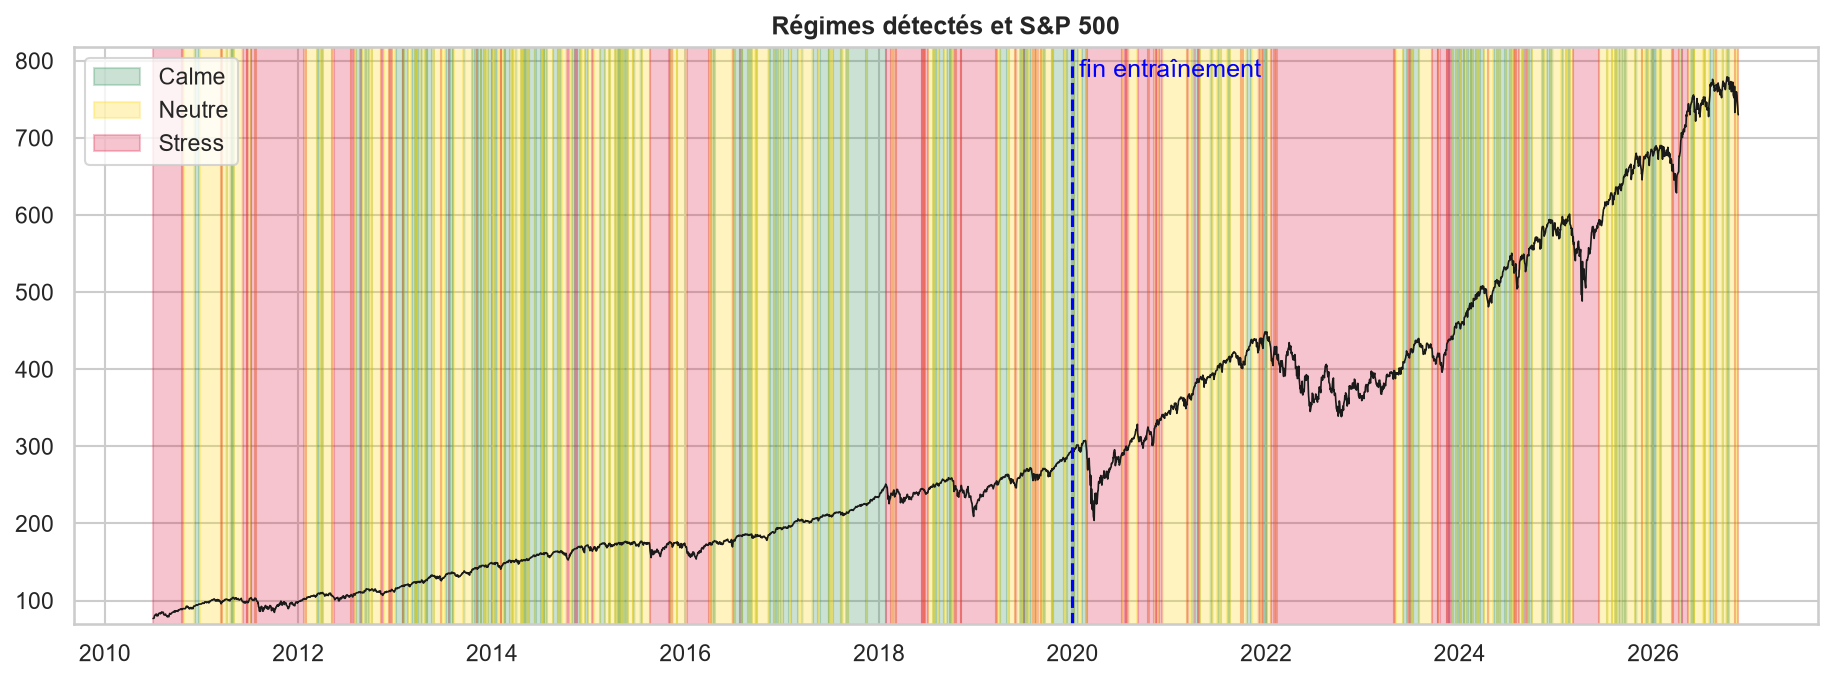
\includegraphics[width=\textwidth]{16_regimes.png}
  \caption{Régimes détectés par le mélange gaussien et cours du S\&P~500.}
  \label{fig:regimes}
\end{figure}

Trois enseignements se dégagent (tableau~\ref{tab:regimes_validation} et figure~\ref{fig:regimes}) :
\begin{itemize}
  \item \textbf{L'agent repère le risque.} Sur les trois périodes, le régime Stress est suivi de la volatilité la plus élevée, et le régime explique 12 à 29 \% de la variance de la volatilité future. Les régimes sont aussi très persistants (la matrice de transition a une diagonale proche de 1), ce qui rend leur détection en temps réel exploitable.
  \item \textbf{Il réagit au risque, il ne l'anticipe pas.} En validation, le régime Calme est suivi d'une volatilité \emph{plus forte} que le régime Neutre. C'est l'effet de février 2020 : le marché était parfaitement calme juste avant le krach de la COVID. Aucune variable de marché ne pouvait annoncer une pandémie ; l'agent bascule en Stress avec quelques jours de retard.
  \item \textbf{Il n'annonce pas de baisse.} Les périodes de stress ont plutôt été suivies de \emph{rebonds} (rendement futur moyen le plus élevé). Réduire systématiquement l'exposition en régime de stress ferait donc souvent vendre au mauvais moment. Ce point sera arbitré sur la validation lors du réglage de l'allocation (section~\ref{sec:allocation_backtest}).
\end{itemize}

\subsection{Les probabilités de régime comme variables de prévision}

Le cours présente une autre utilisation du mélange gaussien : ses probabilités a posteriori $\gamma_{ik}$, ou \og responsabilités \fg{}, peuvent servir de nouvelles variables pour un modèle supervisé. Nous les avons ajoutées aux variables de l'agent Prévision, dans l'idée que certains actifs réagissent différemment selon le régime, puis nous avons comparé les versions avec et sans ces variables par le test de Diebold-Mariano.

Le résultat est négatif. Pour Ridge, l'ajout ne change pas l'erreur de façon significative, ni sur la validation ($p = 0{,}10$) ni sur les prévisions hors pli ($p = 0{,}15$), et la statistique est même légèrement en défaveur de la version enrichie. Pour un arbre peu profond, les prévisions sont strictement identiques : l'arbre n'utilise aucune des trois nouvelles variables. L'information du régime est déjà contenue dans les variables de volatilité et le VIX. Le mélange gaussien sert donc à \emph{décrire} le marché et à gérer le risque, pas à prévoir les rendements relatifs.

\subsection{Agent Alerte : détection d'anomalies}

Une anomalie est une observation rare, qui se distingue nettement de la majorité des données. Ici, c'est une journée de marché anormale : krach, choc de liquidité. L'agent Alerte a deux usages : prévenir le conseiller et le client, et contrôler la qualité des données téléchargées. Nous avons comparé six méthodes du cours :
\begin{itemize}
  \item deux méthodes statistiques sur le rendement du S\&P~500 : le \textbf{z-score} (alerte au-delà de 4 écarts-types) et le \textbf{test de Grubbs}~\cite{grubbs1969}, répété tant qu'il rejette l'hypothèse que la valeur la plus extrême est normale ;
  \item quatre méthodes d'apprentissage sur les cinq variables de marché : la \textbf{gaussienne multivariée} (anomalie si la densité $p(x;\mu,\Sigma)$ est inférieure à un seuil $\epsilon$), l'\textbf{Isolation Forest}~\cite{liu2008} (une anomalie s'isole en peu de coupures aléatoires), le \textbf{LOF}~\cite{breunig2000} (densité locale nettement plus faible que celle des voisins) et la \textbf{One-Class SVM}~\cite{scholkopf2001} (frontière qui entoure les données normales).
\end{itemize}
Les paramètres sont appris sur 2011-2019, avec un taux d'anomalies attendu de 2 \%. L'alerte finale est un \textbf{vote} : elle n'est levée que si au moins trois des quatre méthodes d'apprentissage sont d'accord.

\paragraph{Validation sans étiquettes.} Il n'existe pas de liste officielle des journées anormales. Nous avons donc jugé les détecteurs sur deux critères : retrouvent-ils les crises connues, et s'accordent-ils entre eux ?

\begin{table}[!htb]
  \centering
  \small
  \caption{Détection de six crises connues ($\checkmark$ : au moins une alerte pendant l'épisode).}
  \label{tab:crises}
  \begin{tabular}{@{}l c c c c c c@{}}
    \toprule
    \textbf{Épisode} & \textbf{Gauss.} & \shortstack{\textbf{Isol.}\\\textbf{Forest}} & \textbf{LOF} & \shortstack{\textbf{One-Class}\\\textbf{SVM}} & \shortstack{\textbf{Vote}\\\textbf{$\geq 3/4$}} & \textbf{z-score} \\
    \midrule
    Crise de la dette, août 2011 & $\checkmark$ & $\checkmark$ & $\checkmark$ & $\checkmark$ & $\checkmark$ & $\checkmark$ \\
    Dévaluation du yuan, août 2015 & $\checkmark$ & $\checkmark$ & -- & $\checkmark$ & $\checkmark$ & $\checkmark$ \\
    \og Volmageddon \fg{}, février 2018 & $\checkmark$ & -- & $\checkmark$ & $\checkmark$ & $\checkmark$ & $\checkmark$ \\
    Krach de la COVID, mars 2020 & $\checkmark$ & $\checkmark$ & $\checkmark$ & $\checkmark$ & $\checkmark$ & $\checkmark$ \\
    Choc d'inflation, juin 2022 & $\checkmark$ & $\checkmark$ & $\checkmark$ & $\checkmark$ & $\checkmark$ & $\checkmark$ \\
    Choc de liquidité, août 2024 & $\checkmark$ & -- & $\checkmark$ & $\checkmark$ & $\checkmark$ & -- \\
    \bottomrule
  \end{tabular}
\end{table}

Le vote détecte \textbf{les six crises} (tableau~\ref{tab:crises}), alors que, prises isolément, seules la gaussienne et la One-Class SVM les détectent toutes. Les détecteurs multivariés s'accordent largement entre eux (corrélations de 0,41 à 0,80 entre leurs alertes). Le z-score, en revanche, leur est peu corrélé (0,09 à 0,27) : il repère les chocs brutaux d'une seule journée, alors que les méthodes multivariées repèrent des \emph{états} anormaux qui durent, quand volatilité, VIX et spread de crédit s'élèvent ensemble. Les deux approches sont complémentaires.

\begin{figure}[!htb]
  \centering
  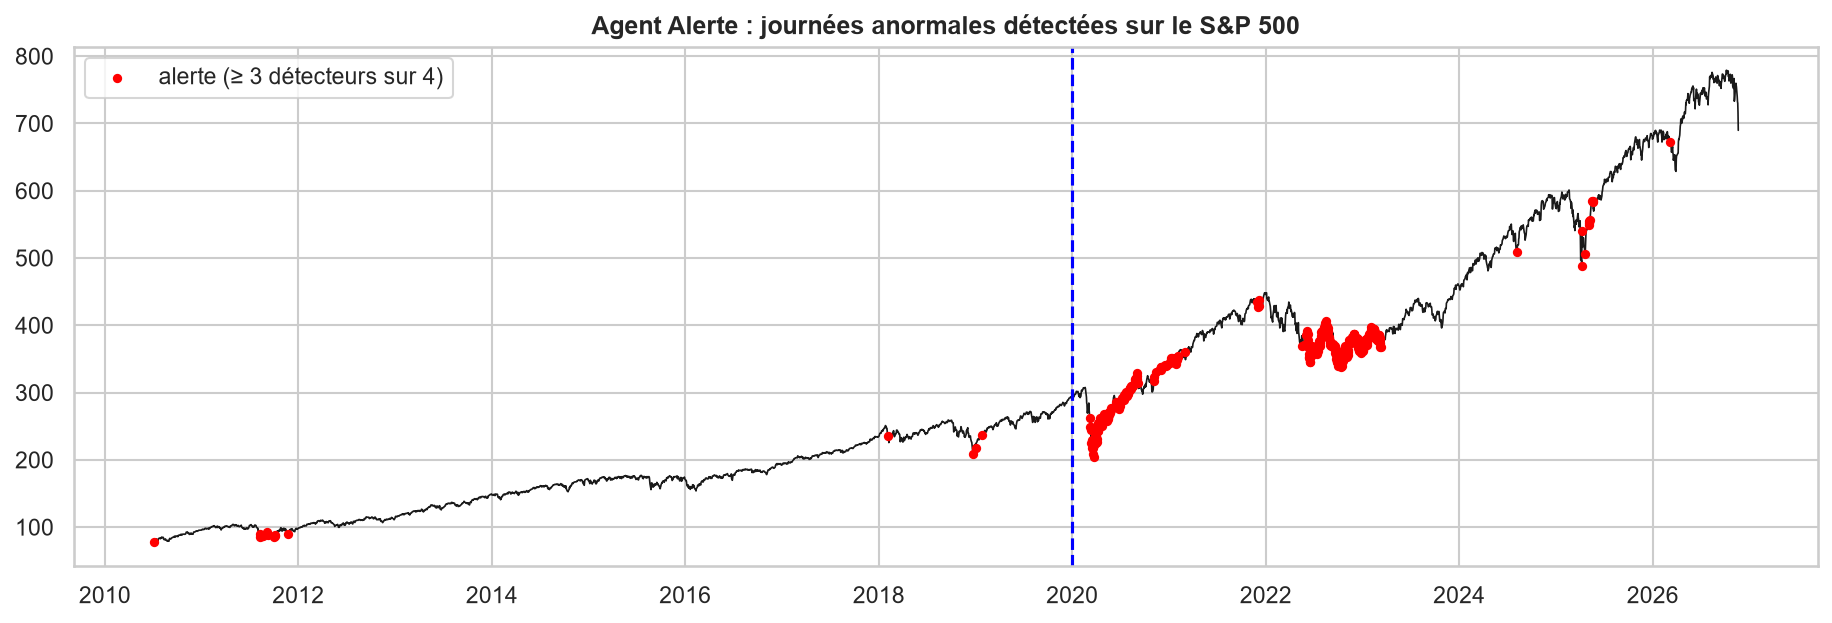
\includegraphics[width=\textwidth]{16b_anomalies.png}
  \caption{Journées signalées par le vote d'au moins trois détecteurs sur quatre. La ligne pointillée marque la fin de l'entraînement.}
  \label{fig:anomalies}
\end{figure}

\paragraph{La dérive des données, encore.} Le vote signale 0,6 \% des jours sur l'entraînement, mais 19 \% après 2019 (figure~\ref{fig:anomalies}) : 2020, puis 2022, ont été bien plus agités que les années 2010. Ce n'est pas une erreur du détecteur : c'est le marché qui a changé. Mais cela montre une limite de tout détecteur appris sur le passé. Pour éviter de banaliser les alertes, il faudrait recalibrer périodiquement les seuils sur des données récentes ; le vote à trois détecteurs sur quatre limite déjà les fausses alertes.
